\section{Related Work}

\textit{Interaction} and \textit{Bayesian Reasoning} are widely studied areas in visualization, but they are typically studied in isolation from each other. This paper focuses on the intersection of these two areas. By using Bayesian reasoning as a test bed for interaction techniques, we add to the body of knowledge on interactive visualizations, and Bayesian reasoning visualizations. The following sections discuss related work studying the value add of interaction, Bayesian reasoning visualizations, and the intersection of the two.

\subsection{Value add of interaction}
Recent work by Dimara and Perin~\cite{dimara2020What} defines interaction (in visualization) as ``the interplay between a person and a data interface involving a data-related intent, at least one action from the person and an interface reaction that is perceived as such.'' Similarly, Yi et al.~\cite{yi2007Toward} and Heer and Shneiderman~\cite{heer2012Interactive} construct taxonomies of interactions for visualization. Others have endeavored to better explain why interaction is useful to visualization from a cognitive processing standpoint~\cite{liu2010Mental, pohl2012User}. In addition to theorizing and categorizing interaction, work has been done designing novel interaction techniques, for example \cite{carpendale2012Beyond, goffin2020Interaction, lee2012Beyond, wybrow2014Interaction},
and identifying how visualization designers can leverage interaction to learn about users and create customized visualizations \cite{brown2012Disfunction, endert2012Semantic}. 

The majority of work on defining, categorizing, theorizing, and leveraging interaction for visualization focuses on visual analytic systems built to help users explore large amounts of data. The value-add of interaction in such cases is relatively clear; actions such as panning, zooming, and selecting subsets are indisputably essential to exploring datasets too large to reasonably fit on a single screen~\cite{wijk2005Value, heer2012Interactive}. Although there are potential costs to interaction~\cite{lam2008Framework, wijk2005Value}, in the case of visual analytic systems, these are often outweighed by benefits. Furthermore, in visual analytic systems interaction is often seen as an essential support for users' cognitive processing; it is viewed as the embodiment of sensemaking and knowledge discovery~\cite{yi2007Toward, pohl2012User, liu2010Mental, pike2009science}.  

In contrast, the value-add of interaction to static visualizations is not clear cut. Here we are specifically referring to interactions that do not reveal otherwise hidden data; i.e. they do not \textit{add} any information to the visualization. For example, Zhi et al.~\cite{zhi2019linking} found that adding interaction through brushing and linking to a storytelling visualization increased engagement. However, they found no measurable impact on comprehension and recall.
Theis et al.~\cite{theis2016Ergonomic} compared static and interactive versions of an uncertainty data visualization and concluded based on accuracy and speed that the static visualization was preferable to its interactive counterpart.
Ragan et al.~\cite{ragan2012Spatial} compared comprehension and detail recall in a pictorial learning activity across interactive versus automatic view controls, and found no significant differences between the two. 
Note that all of these studies include an A-B test between one static and one interactive visualization. Our work adds nuance to this body of work by investigating the value-add of interactivity with a multi-factor experimental design.  
  
\subsection{Bayesian Reasoning}
An area in which Bayesian reasoning problems are prevalent is medical decision making. The standard example of a Bayesian reasoning problem in this context is the mammography problem~\cite{gigerenzer1995How}: 

\textit{The probability of breast cancer is 1\% for women at age forty who participate in routine screening. If a woman has breast cancer, the probability is 80\% that she will get a positive mammography. If a woman does not have breast cancer, the probability is 9.6\% that she will also get a positive mammography.
A woman in this age group had a positive mammography in a routine screening. What is the probability that she actually has breast cancer?}

Using conditional probabilities and Bayesian reasoning to solve this problem is difficult for patients and physicians alike~\cite{eddy1982Probabilistic}. Given the importance of accurate medical risk communication and understanding, numerous studies have investigated how to aid people in Bayesian reasoning. One common approach is to change the text from probability format to frequency format~\cite{gigerenzer1995How, tsai2011Interactive}.    
Another approach is visualization. 

Numerous studies have investigated the effect of visualization on Bayesian reasoning. Different techniques tested include Euler diagrams~\cite{brase2009Pictorial, kellenFacilitating2007, micallef2012Assessing, khan2015Benefits}, frequency grids or icon arrays~\cite{garcia2013Visual, kellenFacilitating2007, micallef2012Assessing, ottley2012Visually, sedlmeier2001Teaching, khan2015Benefits, tsai2011Interactive, bocherer2019How}, decision trees~\cite{friederichs2014Using, sedlmeier2001Teaching, spiegelhalter2011Visualizing, khan2015Benefits, bocherer2019How}, ``beam cut" diagrams~\cite{gigerenzer1995How}, probability curves~\cite{cole1989Understanding}, contingency tables~\cite{cole1989Understanding, cole1989Graphic}, double trees~\cite{khan2015Benefits, khan2018Interactive, bocherer2019How}, flow charts~\cite{khan2015Benefits}, pipe diagrams~\cite{khan2015Benefits}, Sankey diagrams~\cite{khan2015Benefits}, and unit squares~\cite{bocherer2019How}. Despite all of these studies, there is still no clear consensus on the best visualization for Bayesian reasoning. 

Several studies compared multiple Bayesian reasoning visualizations to each other and to text\cite{ottley2016Bayesian, micallef2012Assessing, khan2015Benefits}. All of these studies found that visualization did not significantly improve users' accuracy in performing a Bayesian reasoning task compared to text. Findings from Ottley et al.~and Micallef et al.~indicate that there may be a detrimental effect on users' ability to perform Bayesian reasoning when visualizations and numerical text descriptions are presented together\cite{ottley2016Bayesian, micallef2012Assessing}. Ottley et al.~\cite{ottley2016Bayesian} shed light on a significant performance gap between people with high and low spatial ability on a Bayesian reasoning task, and indicated that optimal visualization and text designs for people with high spatial ability differ from those for people with low spatial ability.

To the best of our knowledge, only two studies have investigated the effect of interactive Bayesian reasoning visualizations, and the results are conflicting. Tsai et al.~\cite{tsai2011Interactive} tested a frequency grid with interactive checkboxes against textual descriptions of the Bayesian reasoning problem. They found the interactive frequency grid resulted in a significant increase in accuracy on a Bayesian reasoning task compared to a textual description of the problem with statistics in probability format. Khan et al.~\cite{khan2018Interactive} compared a static and interactive double tree diagram of the Bayesian reasoning problem. They added interaction via drag and drop, and found the interactive double tree diagram significantly decreased accuracy in performing the Bayesian reasoning task compared to the static version. Our goal is to build off prior work and provide context for conflicting results. By identifying how static visualization design and users' spatial ability affect the value-add of interaction to a static visualization, we can shed light on confounding factors that may explain differences in prior results.
    
\begin{table*}[]
\begin{tabular}{ccccc}
 &  & \multicolumn{3}{c}{\textsc{Base Visualization}} \\ 
 &  & \textit{grouped} & \textit{aligned} & \textit{randomized} \\ 
\multirow{2}{*}{\rotatebox{90}{\textsc{Interaction}}} 
    & \rotatebox{90}{\textit{cbAll}} 
    & 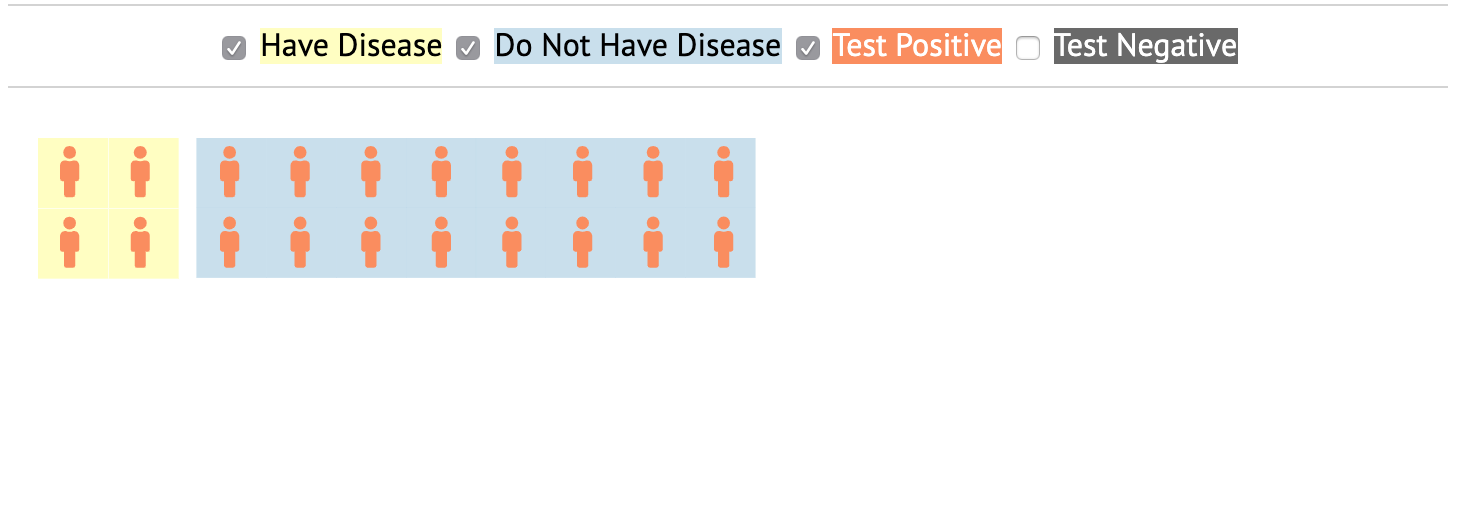
\includegraphics[width=.29\linewidth]{grouped_i.png}
    & 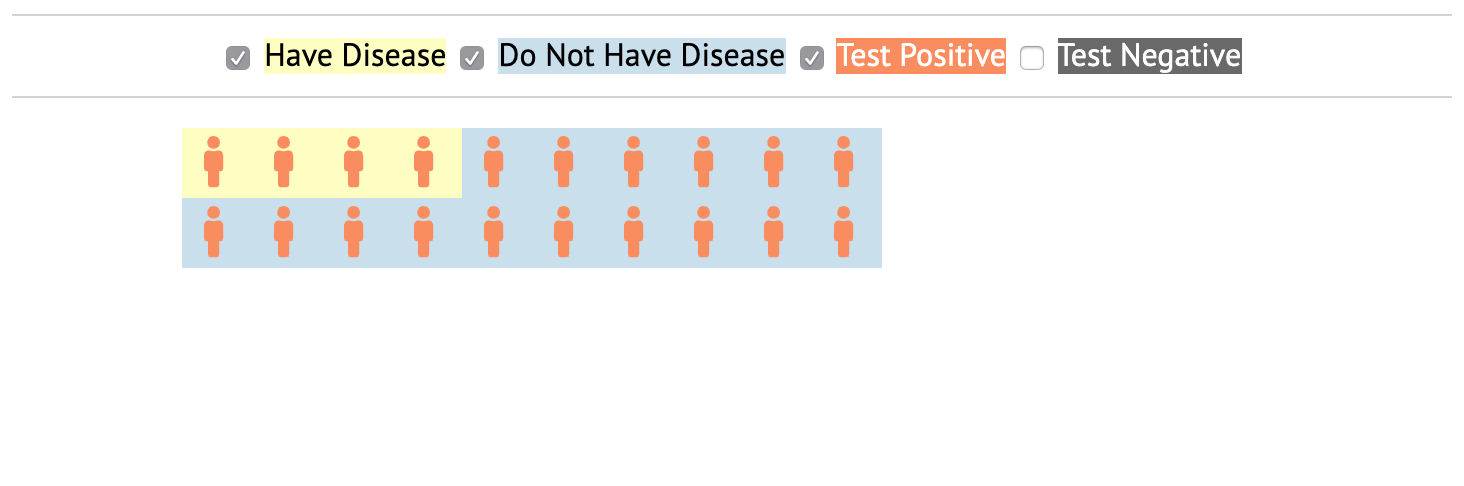
\includegraphics[width=.29\linewidth]{aligned_i.png}  
    & 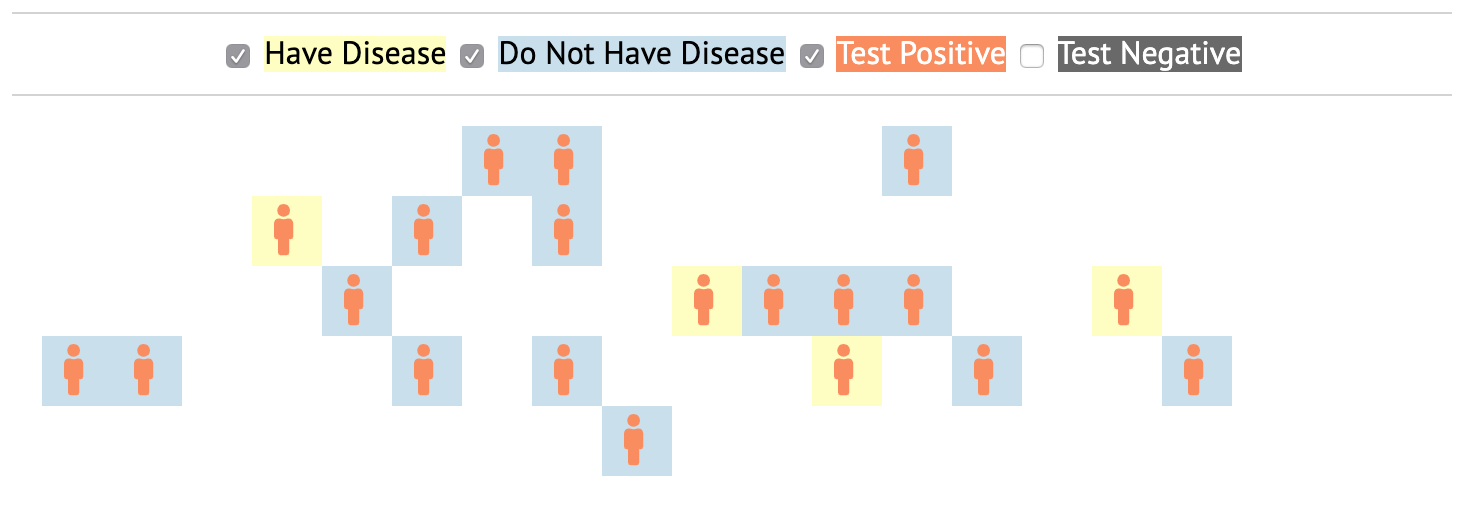
\includegraphics[width=.29\linewidth]{randomized_i.png}
    \\ 
    & \rotatebox{90}{\textit{static}}
    & 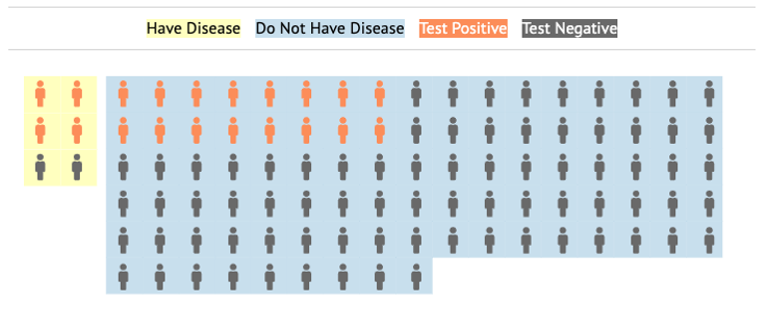
\includegraphics[width=.29\linewidth]{grouped_s.png}
    & 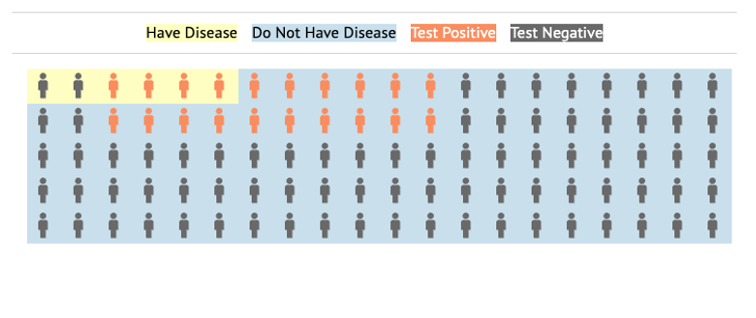
\includegraphics[width=.29\linewidth]{aligned_s.png}  
    & 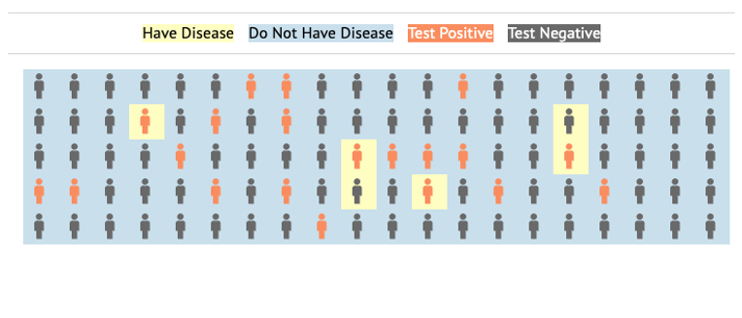
\includegraphics[width=.29\linewidth]{randomized_s.png}
\end{tabular}
\caption{Three interactive and static conditions used in Experiment 1. Full size images are available in supplementary materials.} %\remco{I'm annoyed by the vertical alignment. But after spending two hours digging to latex, I give up! I truly hate latex tables...}}
\label{tab:tabPilotVis}
\end{table*}